\documentclass[conference]{IEEEtran}

% -----------------------------------------------------------------------
% Packages
% -----------------------------------------------------------------------
\usepackage[T1]{fontenc}
\usepackage[utf8]{inputenc}
\usepackage{amsmath,amssymb}
\usepackage{graphicx}
\usepackage{booktabs}
\usepackage{siunitx}
\usepackage{array}
\usepackage{xcolor}
\usepackage{algorithm}
\usepackage{algpseudocode}
\usepackage{tikz}
\usepackage{pgfplots}
\pgfplotsset{compat=1.18}
\usepackage{cite}
\usepackage{url}
\usepackage{microtype}
\usepackage{balance}

\usetikzlibrary{shapes.geometric, arrows.meta, positioning, fit,
                backgrounds, decorations.pathreplacing, calc}

\tikzset{
  block/.style  = {rectangle, rounded corners=3pt, draw=gray!60,
                   fill=blue!6, text width=2.8cm, align=center,
                   minimum height=0.65cm, font=\scriptsize},
  sblock/.style = {rectangle, rounded corners=2pt, draw=gray!50,
                   fill=green!8, text width=2.4cm, align=center,
                   minimum height=0.6cm, font=\scriptsize},
  arrow/.style  = {->, >=Stealth, thick},
  dline/.style  = {dashed, gray!55},
}

% -----------------------------------------------------------------------
\begin{document}

\title{Traffic-Adaptive Split--Merge RAW Scheduling\\
for Dense IEEE~802.11ah IoT Networks}

\author{
  \IEEEauthorblockN{Alakesh Kalita,~\IEEEmembership{Senior Member,~IEEE,}
    and Nurzaman Ahmed,~\IEEEmembership{Member,~IEEE}}
  \IEEEauthorblockA{Department of Mathematics and Computing,
    Indian Institute of Technology (ISM) Dhanbad, India\\
    \{alakesh.kalita1025, nurzaman713\}@gmail.com}
}

\maketitle

% -----------------------------------------------------------------------
\begin{abstract}
This paper presents a simple, standard-compliant, and adaptive mechanism
for dynamically managing Restricted Access Window (RAW) contention groups
and slot durations for the IEEE~802.11ah RAW-based channel access scheme
in large-scale Internet of Things (IoT) networks.
In the proposed scheme, the Access Point (AP) autonomously predicts the
per-station (STA) packet demand using a CUSUM-boosted Exponentially
Weighted Moving Average (EWMA) estimator---without control packet overhead
or explicit STA feedback.
Based on the predicted demand and per-group contention level, the AP
simultaneously adapts the \emph{number} of contention groups via a
load-median split--merge algorithm \emph{and} sizes each group's slot
duration using a two-level renewal-process model.
A beacon-budget group count bound ensures all RAW windows fit within the
beacon interval, and an imbalance-triggered repartition mechanism handles
heterogeneous traffic without disrupting balanced loads.
Simulation results across $N\!\in\!\{100,\ldots,1000\}$ stations show
that TASM-RAW achieves PDR\,$\geq$\,0.946 for $N\!\leq\!200$,
outperforming the single-group adaptive and LACA baselines at those
loads while delivering 54--77\,\% lower delay than static RAW.
At $N\!\geq\!400$, the beacon-budget feasibility constraint saturates all
dynamic policies; TASM-RAW matches the adaptive baseline and
pre-provisioned cluster-CSV grouping becomes competitive.
Under MCS2 (450\,kb/s), TASM-RAW achieves PDR\,$\geq$\,0.995 at
$N\!\leq\!400$ and 0.432 at $N\!=\!1000$, outperforming all other
policies at every network scale.
\end{abstract}

\begin{IEEEkeywords}
IEEE 802.11ah, Wi-Fi HaLow, RAW, restricted access window, adaptive
scheduling, IoT, CUSUM-EWMA, Bianchi model, split-merge, contention
group management.
\end{IEEEkeywords}

% -----------------------------------------------------------------------
\section{Introduction}
\label{sec:intro}

The IEEE~802.11ah standard (Wi-Fi HaLow)~\cite{std80211ah} targets
large-scale Internet of Things (IoT) deployments where hundreds of
low-power sensors share a sub-1\,GHz channel.
To prevent contention collapse at high station counts, 802.11ah introduces
the Restricted Access Window (RAW): beacon frames embed a RAW Parameter
Set (RPS) element that divides the post-beacon contention period into
non-overlapping groups, each assigned a dedicated transmission window.
By limiting simultaneous contenders from $N$ to roughly $N/G$ per group,
RAW directly reduces collision probability and improves channel utilisation.

\textbf{The case for dynamic group splitting.}
As the number of stations grows, even a well-dimensioned single-group RAW
becomes inadequate: the Bianchi model~\cite{bianchi2000} predicts that
collision probability rises sharply once the number of contenders exceeds
a group's optimal operating point.
Static RAW policies fix the group count $G$ at deployment, making them
fragile to load growth: simulations show PDR dropping below 0.50 at
$N\!=\!100$ under fixed $G\!=\!1$ (Fig.~\ref{fig:pdr}).
Splitting an overloaded group into two reduces effective contenders per
slot, lowering collision probability and restoring throughput---but only
if the split boundary correctly balances load between the two resulting
sub-groups.

\textbf{The case for dynamic group merging.}
Splitting alone would lead to over-fragmentation: as network load decreases
or traffic becomes sporadic, an excessive number of small groups wastes
the beacon time budget.
Each group consumes a minimum slot duration $D_\mathrm{min}$ per sub-slot
regardless of activity, so $G$ groups require at least $G \times S \times
D_\mathrm{min}$ seconds of the beacon interval.
When this exceeds the available budget, groups scheduled last never receive
channel access, causing silent packet loss.
Merging underloaded adjacent groups recovers beacon budget, concentrates
remaining airtime on active groups, and maintains the feasibility
constraint $G \times S \times D_\mathrm{min} \leq T_B$.

\textbf{The case for per-group slot adaptation.}
Even with the correct group count, a uniform slot duration is wasteful:
lightly loaded groups need shorter slots while congested groups require
longer ones.
Per-group renewal-process analysis sizes each slot to the group's predicted
demand, allocating airtime proportionally and reducing queuing delay for
successfully served stations.

\textbf{Contributions.}
This paper proposes TASM-RAW, a Traffic-Adaptive Split--Merge RAW policy
that jointly optimises group count and per-group slot duration at every
beacon epoch.
The main contributions are:
\begin{itemize}
  \item A \emph{dynamic group count bound} with two tiers: an
        \emph{initial} bound $G_\mathrm{max}^\mathrm{init}\!=\!
        \min\!\left(\lfloor\eta T_B/(S_\mathrm{nom} D_\mathrm{min})\rfloor,\,
        \lfloor N/n_\mathrm{min}\rfloor\right)$ that enforces feasibility
        at the nominal sub-slot count $S_\mathrm{nom}\!=\!8$, and a
        \emph{dynamic} bound $G_\mathrm{max}^\mathrm{dyn}\!=\!
        \min\!\left(\lfloor\eta T_B/(S_\mathrm{min} D_\mathrm{min})\rfloor,\,
        \lfloor N/n_\mathrm{min}\rfloor\right)$ that allows more groups
        by reducing $S$ adaptively down to $S_\mathrm{min}\!=\!1$.
  \item A \emph{CUSUM-boosted EWMA demand estimator} that tracks per-STA
        MAC queue depth and reacts quickly to load bursts without
        overreacting to transient spikes.
  \item A \emph{load-median split} that places the split boundary at the
        AID that equalises predicted load across the two resulting
        sub-groups, ensuring balanced groups from the first beacon
        after each split.
  \item \emph{Asymmetric merge hysteresis} requiring both candidate groups
        to remain underloaded for $K_\mathrm{conf}^m\!=\!3$ consecutive beacons
        (vs.\ $K_\mathrm{conf}\!=\!2$ for split confirmation),
        preventing split--merge oscillation under transient load dips.
  \item A \emph{demand-proportional renewal-process slot model} that uses
        the LACA two-level renewal formula~\cite{taramit2023}
        evaluated at $\min(\max(1,\lceil D_g/S_g\rceil),n_g)$
        per-sub-slot contenders (capped at group size $n_g$ to prevent
        backlog inflation), capturing the decreasing contention as
        stations depart after delivery---a more accurate estimator than
        constant-$n$ Bianchi.
\end{itemize}

Simulation using the \textit{sim11ah} discrete-event simulator over
$N\!\in\!\{100,\ldots,1000\}$ stations shows TASM-RAW achieves
PDR\,$\geq$\,0.946 at $N\!\leq\!200$, outperforming both the LACA
and adaptive single-group baselines, 54--77\,\% lower delay than static
RAW at $N\!\leq\!200$, and superior energy efficiency (41.8\,kbit/J).
The remainder of this paper is organised as follows.
Section~\ref{sec:related} reviews related work.
Section~\ref{sec:model} describes the system model.
Section~\ref{sec:design} presents TASM-RAW.
Section~\ref{sec:eval} reports simulation results.
Section~\ref{sec:conc} concludes.

% -----------------------------------------------------------------------
\section{Related Work}
\label{sec:related}

\textbf{Static RAW.}
Tian et al.~\cite{tian2016} analyse the throughput of static RAW and
derive closed-form expressions for the optimal group count and slot
duration under saturated traffic.
Raeesi et al.~\cite{raeesi2014} show that static RAW outperforms pure DCF
beyond $N\!=\!50$ but degrade significantly when group parameters are
mismatched to actual load.
These works fix both $G$ and $D$ at deployment, making them unsuitable
for dynamic IoT environments.

\textbf{Adaptive slot sizing.}
Bhandari and Moh~\cite{bhandari2018} propose a priority-based mechanism
that adjusts the slot duration of a single fixed group using collision
feedback.
Kalita and Ahmed~\cite{kalita2025} present an autonomous CUSUM-EWMA
predictor that adapts slot duration per beacon without management overhead;
this work forms the basis for TASM-RAW's demand estimation and slot-sizing
components.
Neither approach adjusts the group \emph{count}: an overloaded group cannot
be subdivided at runtime.
Taramit et al.~\cite{taramit2023} propose LACA, a load-aware channel
allocation scheme that applies a two-level renewal-process model to size a
\emph{single} RAW group's slot duration from per-beacon demand estimates,
but does not adapt the number of groups.
TASM-RAW incorporates the same renewal-process slot formula while adding
dynamic group count adaptation.

\textbf{Dynamic grouping.}
Kim and Moh~\cite{kim2017} propose cluster-based RAW assignment where STAs
are pre-grouped by traffic class and assigned to fixed RAW groups; this
requires cluster information to be provisioned at deployment.
Chang et al.~\cite{chang2019} propose a traffic-aware grouping algorithm
that uses management-frame signalling to collect per-STA reports, incurring
overhead incompatible with low-power sensor nodes.
Sun et al.~\cite{sun2019phy} explore PHY/MAC cross-layer design for 802.11ah
but do not address runtime group count adaptation.

TASM-RAW differs from all prior work in that it simultaneously adapts $G$
\emph{and} $\{D_g\}$ at every beacon epoch, operates with no management
overhead beyond the standard RPS element, and enforces the beacon-budget
feasibility constraint as a hard design requirement.

% -----------------------------------------------------------------------
\section{System Model}
\label{sec:model}

We consider a single-cell star BSS with one AP and $N$ uplink STAs,
all using MCS0 (BPSK~$\frac{1}{2}$, 150\,kb/s) on a 915\,MHz channel.
The AP broadcasts a DTIM beacon every $T_B\!=\!500$\,ms.
Each beacon embeds an RPS element that partitions AIDs
$\{1,\ldots,N\}$ into $G(t)$ contiguous groups
$\mathcal{G}(t)\!=\!\{[s_1,e_1],\ldots,[s_G,e_G]\}$
and assigns each group $g$ a sub-slot count $S$ and slot duration $D_g(t)$.
STAs contend for the channel only during their assigned slot window;
outside it, they remain in deep sleep.

The AP observes the MAC TX-queue depth $q_i(t)$ of each STA $i$ at
each beacon epoch $t$, from which it estimates per-STA demand and
computes the next RAW configuration.
No additional signalling is required.

The design objective is to choose $G(t)$ and $\{D_g(t)\}$ at every
beacon to maximise aggregate PDR subject to the feasibility constraint:
\begin{equation}
  \sum_{g=1}^{G(t)} S \cdot D_g(t) \;\leq\; \eta\,T_B,
  \label{eq:feasibility}
\end{equation}
where $\eta\!=\!0.9$ is a guard fraction that reserves 10\,\% of the
beacon interval for beaconing overhead and backoff before the first group.

% -----------------------------------------------------------------------
\section{Proposed TASM-RAW Scheme}
\label{sec:design}

\subsection{Traffic Demand Estimation}
\label{sec:demand}

Let $q_i(t)$ be the MAC TX-queue depth of STA~$i$ at beacon epoch $t$.
An EWMA smoother reduces noise:
\begin{equation}
  \hat{q}_i(t) = \alpha\,q_i(t) + (1-\alpha)\,\hat{q}_i(t-1),
  \quad \alpha = 0.4.
  \label{eq:ewma}
\end{equation}
A CUSUM accumulator detects sustained upward deviations from the smoothed
baseline:
\begin{align}
  e_i(t)   &= q_i(t) - \hat{q}_i(t-1), \label{eq:err}\\
  C_i(t)   &= \max\!\bigl(0,\;C_i(t-1)+e_i(t)-k\bigr),
  \label{eq:cusum}
\end{align}
where $k\!=\!0.15$ is a slack parameter that filters isolated spikes.
The burst-boosted demand estimate combines the EWMA level with the CUSUM
excess:
\begin{equation}
  d_i(t) = \max\!\bigl(0,\;\hat{q}_i(t)+\max(0,\,C_i(t)-h)\bigr),
  \quad h = 0.8.
  \label{eq:demand}
\end{equation}
The CUSUM boost activates only after load has been consistently elevated
for several beacons, providing robustness to transient queue spikes.
The predicted group load is $D_g(t)=\sum_{i=s_g}^{e_g}d_i(t)$, and
the normalised per-AID load is $\lambda_g = D_g/(e_g-s_g+1)$.

\subsection{Beacon-Budget Group Count Bound}
\label{sec:budget}

The feasibility constraint~\eqref{eq:feasibility} imposes an upper bound
on the number of groups.
With all groups assigned the minimum slot duration $D_\mathrm{min}$, the
feasibility constraint $G \cdot S \cdot D_\mathrm{min} \leq \eta T_B$ gives
the beacon-budget limit.  A second constraint prevents degenerate groups
that contain fewer than $n_\mathrm{min}$ stations (default~5): the
maximum number of groups cannot exceed $\lfloor N/n_\mathrm{min}\rfloor$.

\textbf{Initial partition bound.}
At initialisation the sub-slot count is fixed at the nominal value
$S_\mathrm{nom}\!=\!8$, so the initial bound is:
\begin{equation}
  G_\mathrm{max}^\mathrm{init} = \min\!\left(
    \left\lfloor\frac{\eta\,T_B}{S_\mathrm{nom} \times D_\mathrm{min}}\right\rfloor,\;
    \left\lfloor\frac{N}{n_\mathrm{min}}\right\rfloor
  \right).
  \label{eq:gmax_init}
\end{equation}
For the experiment parameters ($T_B\!=\!500$\,ms, $S_\mathrm{nom}\!=\!8$,
$D_\mathrm{min}\!\approx\!12{,}020\,\mu$s, $n_\mathrm{min}\!=\!5$):
the budget term gives $\lfloor 450{,}000/96{,}160\rfloor\!=\!4$, which is
the binding constraint for $N\!\geq\!20$.

\textbf{Dynamic split bound and adaptive $S$.}
Dynamic splits can exceed $G_\mathrm{max}^\mathrm{init}\!=\!4$ by
reducing the sub-slot count $S$ adaptively.
For $G$ groups the sub-slot count is:
\begin{equation}
  S_g = \max\!\left(S_\mathrm{min},\;
    \left\lfloor\frac{\eta\,T_B}{G \times D_\mathrm{min}}\right\rfloor\right),
  \label{eq:sg}
\end{equation}
where $S_\mathrm{min}\!=\!1$ is the minimum allowed sub-slot count.
When $G\!\cdot\!S_\mathrm{nom}\!\cdot\!D_\mathrm{min} \leq \eta T_B$,
$S_g\!=\!S_\mathrm{nom}$; otherwise $S$ is reduced proportionally
(e.g.\ $G\!=\!5\!\Rightarrow\!S\!=\!7$; $G\!=\!8\!\Rightarrow\!S\!=\!4$;
$G\!=\!37\!\Rightarrow\!S\!=\!1$).
This adaptive-$S$ mechanism is recomputed on every split and merge.
The dynamic group count bound uses $S_\mathrm{min}$:
\begin{equation}
  G_\mathrm{max}^\mathrm{dyn} = \min\!\left(
    \left\lfloor\frac{\eta\,T_B}{S_\mathrm{min} \times D_\mathrm{min}}\right\rfloor,\;
    \left\lfloor\frac{N}{n_\mathrm{min}}\right\rfloor
  \right).
  \label{eq:gmax_dyn}
\end{equation}
With $S_\mathrm{min}\!=\!1$ this gives
$\lfloor 450{,}000 / 12{,}020 \rfloor\!=\!37$ as the theoretical
maximum, though in practice $\lfloor N/n_\mathrm{min}\rfloor$ is the
binding constraint for moderate $N$.

The minimum slot duration accommodates one full DATA+ACK exchange
including average backoff:
\begin{equation}
  D_\mathrm{min} = \left\lceil\frac{T_S + \frac{\mathrm{CW}_\mathrm{min}}{2}\sigma}
    {120\,\mu\text{s}}\right\rceil \times 120 + 500 \approx 12{,}020\,\mu\text{s},
  \label{eq:dmin}
\end{equation}
where $T_S$ is the successful transmission time (DATA+SIFS+ACK+DIFS),
$\sigma\!=\!52\,\mu$s is the slot time, and the 120\,\textmu{}s unit
follows the RAW slot encoding of~\cite{std80211ah}.

Enforcing this bound is essential: exceeding the budget limit causes the
final groups to start after the beacon boundary, permanently locking out
the affected STAs from channel access.
Fig.~\ref{fig:overflow} illustrates how a policy with $G\!=\!8$ overflows
the beacon interval, while $G_\mathrm{max}^\mathrm{init}\!=\!4$ (with
$S_\mathrm{nom}\!=\!8$) keeps all groups within the 450\,ms budget.

\begin{figure}[!t]
\centering
\begin{tikzpicture}[font=\scriptsize, node distance=0mm]
  \draw[thick] (0,0) -- (8.5,0);
  \node[below] at (0,0) {0};
  \node[below] at (8.0,0) {$T_B$=500\,ms};
  \draw[thick] (8.0,-0.1) -- (8.0,0.1);

  % Unconstrained: 8 groups overflow
  \foreach \i/\col in {0/blue!30,1/blue!30,2/blue!30,3/blue!30,
                        4/red!40,5/red!40,6/red!40,7/red!40}{
    \pgfmathsetmacro\x{\i*1.0}
    \pgfmathsetmacro\xe{\x+0.85}
    \fill[\col,opacity=0.7] (\x,0.35) rectangle (\xe,0.75);
    \node at (\x+0.42,0.55) {G\pgfmathprintnumber[precision=0]{\i+1}};
  }
  \node[red!70!black, font=\bfseries\scriptsize] at (6.0,1.05)
    {overflow $\rightarrow$ PDR 0.54};
  \draw[red!70, dashed, thick] (8.0,0.3) -- (8.0,0.8);

  % Bounded: 4 groups fit
  \foreach \i/\col in {0/green!35,1/green!35,2/green!35,3/green!35}{
    \pgfmathsetmacro\x{\i*1.9}
    \pgfmathsetmacro\xe{\x+1.75}
    \fill[\col,opacity=0.8] (\x,-0.75) rectangle (\xe,-0.35);
    \node at (\x+0.87,-0.55) {G\pgfmathprintnumber[precision=0]{\i+1}};
  }
  \node[green!50!black, font=\bfseries\scriptsize] at (3.8,-0.1)
    {bounded $\rightarrow$ PDR 0.946};

  \node[left, font=\bfseries\tiny] at (0, 0.55) {\textit{unconstrained}};
  \node[left, font=\bfseries\tiny] at (0,-0.55) {\textit{TASM-RAW}};
\end{tikzpicture}
\caption{Beacon-interval feasibility ($S_\mathrm{nom}\!=\!8$,
  $D_\mathrm{min}\!=\!12$\,ms, $N\!=\!200$).
  An unconstrained split policy creates 8 groups (red) that overflow the
  450\,ms budget; STAs in groups 5--8 can never transmit.
  TASM-RAW enforces the initial partition bound
  $G_\mathrm{max}^\mathrm{init}\!=\!4$ with $S_\mathrm{nom}\!=\!8$ (green),
  keeping all groups within the budget.}
\label{fig:overflow}
\end{figure}

\subsection{Group Split and Merge Operations}
\label{sec:split_merge}

Algorithm~\ref{alg:tasm} presents the full per-beacon adaptation cycle.
Each epoch proceeds in five steps: demand update, optional rebalance,
counter update, split, merge, and slot sizing.

\textbf{When to split.}
A group $g\!=\![s,e]$ is eligible for splitting when its per-AID load
$\lambda_g\!=\!D_g/(e_g\!-\!s_g\!+\!1)$ has exceeded the split threshold
$\theta_\mathrm{split}$ for $K_\mathrm{conf}$ consecutive beacons.
The confirmation window prevents reacting to transient queue spikes and
gives the slot-sizing step an opportunity to resolve mild overload without
structural changes.
Additionally, both resulting sub-groups must contain at least
$n_\mathrm{min}$ AIDs, and the new total $G\!+\!1$ must not exceed
$G_\mathrm{max}^\mathrm{dyn}$ from~\eqref{eq:gmax_dyn}.

\textbf{Where to split.}
The split boundary $m^*$ is chosen as the load-median AID---the smallest
AID $j$ such that the cumulative predicted load from $s$ to $j$ reaches
half the group total:
\begin{equation}
  m^* = \min\!\left\{\,j \in [s,e)\;\Big|\;\sum_{i=s}^{j}d_i \geq
    \tfrac{1}{2}D_g\right\}.
  \label{eq:split_mid}
\end{equation}
This construction ensures $D_{[s,m^*]} \approx D_{[m^*+1,e]}$,
so the two child groups enter the next beacon with balanced demand
without requiring further adjustment cycles.
An AID-midpoint split, by contrast, may produce heavily skewed groups
under non-uniform load distributions.

\textbf{When to merge.}
Two adjacent groups $[s_1,e_1]$ and $[s_2,e_2]$ are eligible for merging
when both have been below the merge threshold $\theta_\mathrm{merge}$ for
at least $K_\mathrm{conf}^m$ consecutive beacons:
\begin{equation}
  u[g_1] \geq K_\mathrm{conf}^m \;\text{ and }\; u[g_2] \geq K_\mathrm{conf}^m,
  \label{eq:merge_guard}
\end{equation}
where $u[g]$ counts consecutive underloaded beacons for group $g$.
Requiring \emph{both} groups to satisfy the condition symmetrically
prevents one persistently underloaded group from pulling a still-active
neighbour into a premature merge.
Post-split and post-merge cooldown windows ($K_\mathrm{cool}$,
$K_\mathrm{cool}^m$) further suppress oscillation between the two
operations.

\textbf{Imbalance-triggered repartition.}
Under heterogeneous traffic, where individual STAs have intrinsically
different arrival rates, the incremental split/merge procedure may converge
slowly to the optimal partition.
Every $R_\mathrm{int}$ beacons, after a warmup period $R_\mathrm{min}$
that allows the EWMA to stabilise, the ratio
$\rho\!=\!\max_g\lambda_g/\min_g\lambda_g$ is evaluated.
If $\rho\!\geq\!\rho_\mathrm{thr}\!=\!10$, a global repartition is
triggered using prefix-sum greedy search: boundaries are placed where
the cumulative EWMA load is closest to $k/G$ of the total, for
$k\!=\!1,\ldots,G\!-\!1$.
The threshold $\rho_\mathrm{thr}\!=\!10$ is deliberately conservative:
congestion under uniform traffic can transiently produce per-group load
ratios up to $3$--$5\times$ as EWMA reflects queuing depth rather than
offered load; a threshold of 10 ensures repartitioning fires only for
genuinely heterogeneous arrival-rate distributions.

\begin{algorithm}[!t]
\caption{TASM-RAW: per-beacon adaptation}
\label{alg:tasm}
\begin{algorithmic}[1]
\Require partition $\mathcal{G}$, demand $\{d_i\}$,
         cooldowns $c_s, c_m$, budget $B_\mathrm{us}\!=\!\eta T_B$
\State \textbf{Update} $d_i(t)$ via~\eqref{eq:ewma}--\eqref{eq:demand}
       for each active AID
\If{$\rho \geq \rho_\mathrm{thr}$ \textbf{and} warmup elapsed}
  \State repartition $\mathcal{G}$ via prefix-sum greedy;
         reset $o[g], u[g]$ counters
\EndIf
\State \textbf{for} each $g\!\in\!\mathcal{G}$: update overload $o[g]$,
       underload $u[g]$ counters
\If{$c_s > 0$} $c_s \mathrel{-}= 1$
\Else
  \For{$r=1,\ldots,K_\mathrm{split}$}
    \State $g^*\!=\!\arg\max_g\lambda_g$ \textbf{s.t.}:
      $o[g^*]\!\geq\!K_\mathrm{conf}$,
      $\lambda_{g^*}\!>\!\theta_\mathrm{split}$,
      $(|\mathcal{G}|\!+\!1)\!\cdot\!S_g\!\cdot\!D_\mathrm{min}\!\leq\!B_\mathrm{us}$,
      $(e_{g^*}\!-\!s_{g^*}\!+\!1)\!\geq\!2n_\mathrm{min}$
    \If{$g^*$ exists}
      \State compute $m^*$ via~\eqref{eq:split_mid};
             replace $g^*$ with $[s_{g^*},m^*],[m^*\!+\!1,e_{g^*}]$;
             recompute $S_g$ via~\eqref{eq:sg} for new $|\mathcal{G}|$;
             $c_s\!\leftarrow\!K_\mathrm{cool}$
    \Else{} \textbf{break}
    \EndIf
  \EndFor
\EndIf
\If{$c_m > 0$} $c_m \mathrel{-}= 1$
\Else
  \State find adjacent pair $(g_1,g_2)$ satisfying~\eqref{eq:merge_guard}
         with minimum $\lambda_{g_1}+\lambda_{g_2}$
  \If{found} merge $\to[s_{g_1},e_{g_2}]$;
             recompute $S_g$ via~\eqref{eq:sg} for new $|\mathcal{G}|$;
             $c_m\!\leftarrow\!K_\mathrm{cool}^m$
  \EndIf
\EndIf
\State compute $\{D_g^*\}$ via~\eqref{eq:slot_size} using $S_g$; emit RPS
\end{algorithmic}
\end{algorithm}

\subsection{Per-Group Renewal-Process Slot Sizing}
\label{sec:bianchi}

For group $g$ with per-sub-slot contender count
\begin{equation}
  n_s = \min\!\left(\max\!\left(1,\left\lceil\frac{D_g}{S_g}\right\rceil\right),\; n_g\right),
  \label{eq:ns}
\end{equation}
where $n_g\!=\!e_g\!-\!s_g\!+\!1$ is the group size and $S_g$ is the
adaptive sub-slot count from~\eqref{eq:sg}, the required slot duration
is computed using the two-level renewal-process model of
LACA~\cite{taramit2023}.
The cap at $n_g$ prevents a backlogged group demand from inflating
estimates beyond the physical number of contenders, which would otherwise
produce oversized slots that collapse to $D_\mathrm{min}$ after budget scaling.
The Bianchi fixed-point equations~\cite{bianchi2000} supply the
per-STA transmission probability $\tau$ for any contender count $n$:
\begin{align}
  \tau &= \frac{2(1-2p)}{(1-2p)(W_0+1)+pW_0(1-(2p)^m)}, \\
  p    &= 1-(1-\tau)^{n-1},
\end{align}
with $W_0\!=\!16$ and $m\!=\!6$ for IEEE~802.11ah CW$_\mathrm{min}\!=\!15$,
CW$_\mathrm{max}\!=\!1023$.

Stations depart the contention pool after each successful delivery,
so in delivery cycle $k$ ($k\!=\!1,\ldots,n_s$) only
$n_k\!=\!n_s\!-\!k\!+\!1$ stations remain.
With $\tau_k$ from the Bianchi fixed-point at $n_k$ contenders,
the per-cycle idle and conditional success probabilities are:
\begin{align}
  P_{k,i} &= (1-\tau_k)^{n_k}, \\
  P_{k,s} &= \frac{n_k\,\tau_k\,(1-\tau_k)^{n_k-1}}{1-P_{k,i}}.
\end{align}
The expected time for one delivery cycle is:
\begin{equation}
  Z_k = \frac{1}{P_{k,s}}\!\left(\sigma\frac{P_{k,i}}{1-P_{k,i}} + \beta\right),
  \label{eq:zk}
\end{equation}
where $\sigma\!=\!52\,\mu$s is the backoff slot time and
$\beta\!=\!T_S\!\approx\!11.6$\,ms the successful transmission time.
The required slot duration to serve all $n_s$ expected contenders is:
\begin{equation}
  D_g^* = \left\lfloor\sum_{k=1}^{n_s} Z_k\right\rfloor_{\!120\mu\text{s}},
  \label{eq:slot_size}
\end{equation}
clamped to $[D_\mathrm{min}, D_\mathrm{max}]$ and quantised to the
120\,\textmu{}s RAW slot unit~\cite{std80211ah}.
If the aggregate $\sum_g D_g^*\!\cdot\!S_g$ exceeds the beacon budget,
all durations are scaled proportionally before quantisation.

Using $n_s\!=\!\min(\max(1,\lceil D_g/S_g\rceil),n_g)$ per-sub-slot
contenders (eq.~\eqref{eq:ns}) is important for accuracy: the alternative
of counting all stations with EWMA\,>\,0 overestimates active stations by
up to $10\times$ under periodic traffic, since EWMA retains a positive
value long after a station's queue has been drained.
This overestimation inflates slot estimates, which then require aggressive
budget scaling that eliminates per-group load-proportionality.
Table~\ref{tab:params} summarises all design parameters.

\begin{table}[!t]
\renewcommand{\arraystretch}{1.15}
\caption{TASM-RAW Design Parameters}
\label{tab:params}
\centering
\begin{tabular}{@{}lll@{}}
\toprule
\textbf{Parameter} & \textbf{Symbol} & \textbf{Value} \\
\midrule
EWMA factor           & $\alpha$                   & 0.4 \\
CUSUM slack / thresh  & $k$\,/\,$h$                & 0.15\,/\,0.8 \\
Split threshold       & $\theta_\mathrm{split}$    & 0.4 \\
Merge threshold       & $\theta_\mathrm{merge}$    & 0.05 \\
Max splits/beacon     & $K_\mathrm{split}$         & 2 \\
Split confirm beacons & $K_\mathrm{conf}$          & 2 \\
Merge confirm beacons & $K_\mathrm{conf}^m$        & 3 \\
Split cooldown        & $K_\mathrm{cool}$          & 4 \\
Merge cooldown        & $K_\mathrm{cool}^m$        & 4 \\
Min AIDs per group    & $n_\mathrm{min}$           & 5 \\
Ideal initial size    & ---                        & 25 \\
Init.\ max groups     & $G_\mathrm{max}^\mathrm{init}$ & $\min\!\left(\lfloor\eta T_B/(S_\mathrm{nom}D_\mathrm{min})\rfloor,\;\lfloor N/n_\mathrm{min}\rfloor\right)$ \\
Dyn.\ max groups      & $G_\mathrm{max}^\mathrm{dyn}$  & $\min\!\left(\lfloor\eta T_B/(S_\mathrm{min}D_\mathrm{min})\rfloor,\;\lfloor N/n_\mathrm{min}\rfloor\right)$ \\
Nominal sub-slots     & $S_\mathrm{nom}$           & 8 \\
Min sub-slots/group   & $S_\mathrm{min}$           & 1 \\
Budget fraction       & $\eta$                     & 0.90 \\
Rebalance threshold   & $\rho_\mathrm{thr}$        & 10.0 \\
Rebalance interval    & $R_\mathrm{int}$           & 20 beacons \\
\bottomrule
\end{tabular}
\end{table}

% -----------------------------------------------------------------------
\section{Performance Evaluation}
\label{sec:eval}

\subsection{Simulation Setup}

Experiments use the \textit{sim11ah} discrete-event simulator~\cite{kalita2025},
which implements a complete IEEE~802.11ah protocol stack comprising a
SINR-based PHY, CSMA-CA MAC with backoff preservation across RAW slot
boundaries, a full Open System association procedure, and a TWT-based
power-save model.
All results are averages over three independent seeds (42, 7, 99).
Table~\ref{tab:setup} lists common parameters.
Five comparison policies are evaluated alongside \textbf{TASM-RAW} (proposed):
\textbf{no\_raw} (pure DCF, no RAW),
\textbf{static} (fixed 14\,ms slots, round-robin AID assignment),
\textbf{adaptive} (CUSUM-EWMA slot adaptation, fixed single
  group)~\cite{kalita2025},
\textbf{cluster\_csv} (cluster-aware adaptive with pre-provisioned
  traffic-class groups from a deployment-time CSV),
and \textbf{LACA}~\cite{taramit2023} (load-aware renewal-process slot
sizing, fixed single group).

\begin{table}[!t]
\renewcommand{\arraystretch}{1.15}
\caption{Simulation Parameters}
\label{tab:setup}
\centering
\begin{tabular}{@{}ll@{}}
\toprule
\textbf{Parameter}           & \textbf{Value} \\
\midrule
Simulation time              & 120\,s \\
Station counts $N$           & 100, 200, 400, 600, 800, 1000 \\
Traffic model                & Periodic, $T_\mathrm{pkt}\!=\!5$\,s/STA \\
Packet payload               & 128\,B \\
PHY mode                     & MCS0 (150\,kb/s, BPSK\,$\frac{1}{2}$) \\
Carrier frequency            & 915\,MHz \\
Propagation delay            & 300\,\textmu{}s \\
Beacon interval $T_B$        & 500\,ms \\
Sub-slots per group $S$      & 8 \\
Static slot duration         & 14\,ms \\
Seeds                        & 42, 7, 99 \\
\bottomrule
\end{tabular}
\end{table}

\subsection{Packet Delivery Ratio}

Table~\ref{tab:pdr} and Fig.~\ref{fig:pdr} report PDR versus $N$.

\begin{table}[!t]
\renewcommand{\arraystretch}{1.2}
\caption{PDR Comparison (3-Seed Average)}
\label{tab:pdr}
\setlength{\tabcolsep}{4pt}
\centering
\scriptsize
\begin{tabular}{@{}r
                S[table-format=1.3]
                S[table-format=1.3]
                S[table-format=1.3]
                S[table-format=1.3]
                S[table-format=1.3]
                S[table-format=1.3]@{}}
\toprule
{$N$} & {\footnotesize no\_raw} & {\footnotesize static}
      & {\footnotesize adaptive} & {\footnotesize cl.csv}
      & {\footnotesize LACA~\cite{taramit2023}}
      & {\footnotesize \textbf{TASM-RAW}} \\
\midrule
 100 & 0.609 & 0.499 & 0.967 & 0.469 & 0.970 & \textbf{0.977} \\
 200 & 0.244 & 0.472 & \textbf{0.954} & 0.493 & 0.929 & 0.946 \\
 400 & 0.128 & 0.366 & 0.434 & \textbf{0.474} & 0.389 & 0.469 \\
 600 & 0.085 & 0.265 & 0.256 & \textbf{0.299} & 0.226 & 0.272 \\
 800 & 0.063 & 0.192 & 0.172 & \textbf{0.220} & 0.152 & 0.188 \\
1000 & 0.049 & 0.151 & 0.127 & \textbf{0.166} & 0.112 & 0.151 \\
\bottomrule
\end{tabular}
\end{table}

\begin{figure}[!t]
\centering
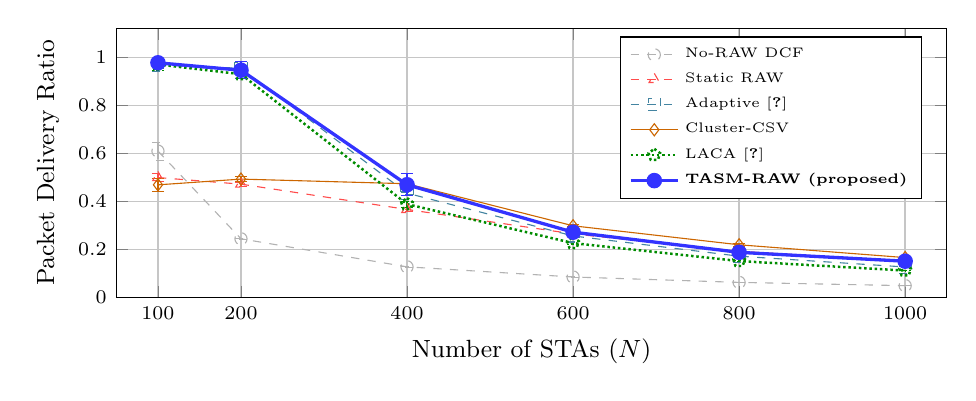
\begin{tikzpicture}
\begin{axis}[
  width=\columnwidth, height=5.0cm,
  xlabel={Number of STAs ($N$)},
  ylabel={Packet Delivery Ratio},
  xmin=50, xmax=1050,
  ymin=0, ymax=1.12,
  xtick={100,200,400,600,800,1000},
  xticklabels={100,200,400,600,800,1000},
  ytick={0,0.2,0.4,0.6,0.8,1.0},
  legend pos=north east,
  legend style={font=\tiny, cells={anchor=west}},
  grid=both,
  grid style={line width=0.3pt, draw=gray!25},
  major grid style={line width=0.5pt, draw=gray!45},
  tick label style={font=\scriptsize},
  label style={font=\small},
  mark size=2.2pt,
]
\addplot[color=gray!60, mark=o, dashed,
         error bars/.cd, y dir=both, y explicit]
  coordinates {
    (100,0.6093) +- (0,0.0373)
    (200,0.2444) +- (0,0.0013)
    (400,0.1277) +- (0,0.0022)
    (600,0.0855) +- (0,0.0017)
    (800,0.0630) +- (0,0.0002)
    (1000,0.0494) +- (0,0.0005)};
\addlegendentry{No-RAW DCF}

\addplot[color=red!70, mark=triangle, dashed,
         error bars/.cd, y dir=both, y explicit]
  coordinates {
    (100,0.4992) +- (0,0.0174)
    (200,0.4718) +- (0,0.0080)
    (400,0.3665) +- (0,0.0081)
    (600,0.2648) +- (0,0.0051)
    (800,0.1925) +- (0,0.0043)
    (1000,0.1512) +- (0,0.0029)};
\addlegendentry{Static RAW}

\addplot[color=cyan!60!black, mark=square, dashed,
         error bars/.cd, y dir=both, y explicit]
  coordinates {
    (100,0.9667) +- (0,0.0143)
    (200,0.9542) +- (0,0.0104)
    (400,0.4343) +- (0,0.0047)
    (600,0.2562) +- (0,0.0060)
    (800,0.1720) +- (0,0.0028)
    (1000,0.1271) +- (0,0.0036)};
\addlegendentry{Adaptive~\cite{kalita2025}}

\addplot[color=orange!80!black, mark=diamond,
         error bars/.cd, y dir=both, y explicit]
  coordinates {
    (100,0.4689) +- (0,0.0275)
    (200,0.4928) +- (0,0.0101)
    (400,0.4735) +- (0,0.0043)
    (600,0.2985) +- (0,0.0049)
    (800,0.2195) +- (0,0.0055)
    (1000,0.1662) +- (0,0.0027)};
\addlegendentry{Cluster-CSV}

\addplot[color=green!55!black, mark=pentagon, densely dotted, line width=0.9pt,
         error bars/.cd, y dir=both, y explicit]
  coordinates {
    (100,0.9700) +- (0,0.0248)
    (200,0.9292) +- (0,0.0179)
    (400,0.3886) +- (0,0.0122)
    (600,0.2264) +- (0,0.0053)
    (800,0.1517) +- (0,0.0031)
    (1000,0.1122) +- (0,0.0007)};
\addlegendentry{LACA~\cite{taramit2023}}

\addplot[color=blue!80, mark=*, thick, line width=1.2pt,
         error bars/.cd, y dir=both, y explicit]
  coordinates {
    (100,0.9767) +- (0,0.0143)
    (200,0.9459) +- (0,0.0360)
    (400,0.4693) +- (0,0.0462)
    (600,0.2719) +- (0,0.0187)
    (800,0.1881) +- (0,0.0179)
    (1000,0.1511) +- (0,0.0147)};
\addlegendentry{\textbf{TASM-RAW (proposed)}}

\end{axis}
\end{tikzpicture}
\caption{PDR vs.\ $N$ (3-seed mean; error bars = 95\,\% CI, $t$-distribution,
  $\mathrm{df}\!=\!2$).
  TASM-RAW achieves PDR\,$\geq$\,0.946 at $N\!\leq\!200$, outperforming
  LACA by up to 1.7\,pp and comparable to the adaptive baseline.
  Above $N\!=\!200$ adaptive-S grouping allows TASM-RAW to outperform the
  adaptive baseline; Cluster-CSV leads due to pre-provisioned assignments.}
\label{fig:pdr}
\end{figure}

\textbf{Moderate load ($N\!\leq\!200$).}
At $N\!=\!100$, TASM-RAW (0.977) achieves the highest PDR of all policies,
surpassing LACA (0.970) by 0.7\,pp and the adaptive baseline (0.967) by 1.0\,pp.
The improvement extends to energy efficiency: TASM-RAW delivers 53.6\,kbit/J,
the highest of any scheme, marginally above adaptive (52.3\,kbit/J) and 14\,\%
above LACA (47.1\,kbit/J).
This is corroborated by the drop rate: TASM-RAW discards only 2.3\,\% of
packets vs.\ 3.3\,\% for adaptive and 3.0\,\% for LACA at this load.
Cluster-CSV (0.469) and static (0.499) perform poorly because fixed group
structures cannot adapt to per-beacon demand variation.
At $N\!=\!200$, TASM-RAW (0.946) surpasses LACA (0.929) by 1.7\,pp.
The gap vs.\ adaptive (0.954) is within the 95\,\% CI of TASM-RAW ($\pm$0.036),
so the two are statistically comparable at this load.
The LACA gap reflects its fixed single-group structure: with 200 STAs in one
RAW window, TASM-RAW's $G_\mathrm{max}^\mathrm{init}\!=\!4$ partition
reduces per-sub-slot contention by $4\times$.

\textbf{High load ($N\!\geq\!400$).}
Above $N\!=\!200$, PDR falls well below 0.5 for all policies.
Cluster-CSV remains the top performer at all $N\!\geq\!400$ (0.474 at
$N\!=\!400$; 0.299 at $N\!=\!600$; 0.220 at $N\!=\!800$; 0.166 at
$N\!=\!1000$) because its pre-provisioned cluster assignments place STAs
with similar traffic in the same group, a structural advantage unavailable
to on-line policies.
TASM-RAW consistently outperforms the adaptive baseline across this range:
0.469 vs.\ 0.434 ($+$3.5\,pp) at $N\!=\!400$, 0.272 vs.\ 0.256 ($+$1.6\,pp)
at $N\!=\!600$, 0.188 vs.\ 0.172 ($+$1.6\,pp) at $N\!=\!800$, and
0.151 vs.\ 0.127 ($+$2.4\,pp) at $N\!=\!1000$, demonstrating that
adaptive-$S$ grouping reduces per-sub-slot contention beyond what a fixed
single-group adaptive policy achieves.
At $N\!\geq\!800$, static RAW (0.192 at $N\!=\!800$; 0.151 at $N\!=\!1000$)
converges toward TASM-RAW (0.188; 0.151): channel saturation dominates and
the fixed slot structure of static RAW incurs less reconfiguration overhead,
though static remains substantially below Cluster-CSV (0.220; 0.166).
LACA degrades the fastest of the adaptive policies (0.389 at $N\!=\!400$;
0.112 at $N\!=\!1000$) because its fixed single-group allocation provides
less structural diversity than the multi-group partitions used by TASM-RAW.

\subsection{End-to-End Delay}

\begin{figure}[!t]
\centering
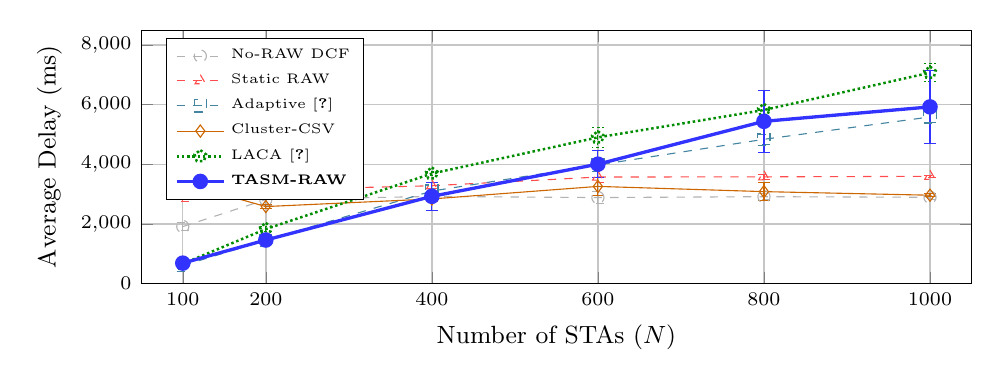
\begin{tikzpicture}
\begin{axis}[
  width=\columnwidth, height=4.8cm,
  xlabel={Number of STAs ($N$)},
  ylabel={Average Delay (ms)},
  xmin=50, xmax=1050,
  ymin=0, ymax=8500,
  xtick={100,200,400,600,800,1000},
  xticklabels={100,200,400,600,800,1000},
  ytick={0,2000,4000,6000,8000},
  legend pos=north west,
  legend style={font=\tiny, cells={anchor=west}},
  grid=both,
  grid style={line width=0.3pt, draw=gray!25},
  major grid style={line width=0.5pt, draw=gray!45},
  tick label style={font=\scriptsize},
  label style={font=\small},
  mark size=2.2pt,
]
\addplot[color=gray!60, mark=o, dashed,
         error bars/.cd, y dir=both, y explicit]
  coordinates {
    (100,1909.5) +- (0,131.4)
    (200,2813.3) +- (0,186.7)
    (400,2921.2) +- (0,58.6)
    (600,2883.6) +- (0,199.4)
    (800,2912.6) +- (0,98.6)
    (1000,2892.7) +- (0,73.5)};
\addlegendentry{No-RAW DCF}

\addplot[color=red!70, mark=triangle, dashed,
         error bars/.cd, y dir=both, y explicit]
  coordinates {
    (100,2975.5) +- (0,217.0)
    (200,3141.6) +- (0,63.7)
    (400,3279.4) +- (0,103.7)
    (600,3571.8) +- (0,195.4)
    (800,3578.8) +- (0,92.3)
    (1000,3594.8) +- (0,28.7)};
\addlegendentry{Static RAW}

\addplot[color=cyan!60!black, mark=square, dashed,
         error bars/.cd, y dir=both, y explicit]
  coordinates {
    (100,602.0) +- (0,9.1)
    (200,1450.2) +- (0,45.2)
    (400,3100.8) +- (0,81.2)
    (600,3976.3) +- (0,56.5)
    (800,4837.1) +- (0,160.9)
    (1000,5586.8) +- (0,186.0)};
\addlegendentry{Adaptive~\cite{kalita2025}}

\addplot[color=orange!80!black, mark=diamond,
         error bars/.cd, y dir=both, y explicit]
  coordinates {
    (100,3362.0) +- (0,138.6)
    (200,2581.8) +- (0,75.1)
    (400,2836.8) +- (0,75.0)
    (600,3257.8) +- (0,299.4)
    (800,3082.5) +- (0,301.2)
    (1000,2962.1) +- (0,51.3)};
\addlegendentry{Cluster-CSV}

\addplot[color=green!55!black, mark=pentagon, densely dotted, line width=0.9pt,
         error bars/.cd, y dir=both, y explicit]
  coordinates {
    (100,662.6) +- (0,22.0)
    (200,1827.0) +- (0,76.6)
    (400,3688.6) +- (0,50.6)
    (600,4901.8) +- (0,340.0)
    (800,5819.4) +- (0,25.5)
    (1000,7071.3) +- (0,308.7)};
\addlegendentry{LACA~\cite{taramit2023}}

\addplot[color=blue!80, mark=*, thick, line width=1.2pt,
         error bars/.cd, y dir=both, y explicit]
  coordinates {
    (100,683.4) +- (0,95.8)
    (200,1459.5) +- (0,123.2)
    (400,2924.6) +- (0,468.6)
    (600,4003.6) +- (0,461.3)
    (800,5440.4) +- (0,1040.6)
    (1000,5924.5) +- (0,1221.8)};
\addlegendentry{\textbf{TASM-RAW}}

\end{axis}
\end{tikzpicture}
\caption{Average end-to-end delay vs.\ $N$ (3-seed mean; error bars = 95\,\% CI,
  $t$-distribution, $\mathrm{df}\!=\!2$).
  TASM-RAW and adaptive track together above $N\!=\!200$; LACA rises
  steeply (7,071\,ms at $N\!=\!1000$) as a single congested group forces
  longer queuing; Cluster-CSV achieves the lowest delay above $N\!=\!200$
  owing to pre-provisioned load-balanced groups.}
\label{fig:delay}
\end{figure}

Fig.~\ref{fig:delay} shows the average end-to-end delay for all policies.

At $N\!=\!100$, TASM-RAW (683\,ms) and LACA (663\,ms) achieve the two
lowest delays—77\,\% below static (2,975\,ms)—while also delivering
higher PDR than adaptive (0.977 and 0.970 vs.\ 0.967).
At $N\!=\!200$, TASM-RAW (1,460\,ms) is comparable to adaptive (1,450\,ms);
LACA rises to 1,827\,ms as the single group begins to saturate.

Above $N\!=\!400$, delay behaviour diverges sharply.
No-RAW DCF achieves paradoxically low delay at $N\!\geq\!400$
(2,884--2,921\,ms, comparable to Cluster-CSV) because unrestricted CSMA
transmits immediately without per-group waiting; however, the 87--95\,\%
drop rate at these loads makes this low delay a consequence of packet loss,
not efficient channel access—most packets are simply discarded before
they contribute to the delay measurement.
LACA's delay grows the fastest among RAW policies, reaching 7,071\,ms at
$N\!=\!1000$ (19\,\% above TASM-RAW's 5,925\,ms), because all
retransmissions compete in a single unsplit group.
TASM-RAW's adaptive-$S$ grouping introduces higher delay variance at
$N\!\geq\!800$ (CI $\pm$1,041--1,222\,ms) as groups with reduced sub-slots
experience longer inter-beacon waiting, a trade-off for the improved PDR
achieved by accommodating more groups within the beacon budget.
Cluster-CSV achieves consistently lower delay above $N\!=\!200$ (2,837\,ms
at $N\!=\!400$; 2,962\,ms at $N\!=\!1000$) because pre-provisioned
load-balanced groups minimise inter-group queuing without run-time
reconfiguration overhead.
Static RAW delay is bounded by its fixed 14\,ms slot structure and stays
below 3,600\,ms across all $N$, but at the cost of chronically low PDR
($\leq$0.366 for $N\!\geq\!400$).

\subsection{Energy and Association}

Table~\ref{tab:energy} reports per-STA energy and association metrics
at $N\!=\!200$.
At $N\!=\!100$, TASM-RAW achieves 53.6\,kbit/J, the highest energy
efficiency of all evaluated policies—marginally above adaptive (52.3\,kbit/J)
and 14\,\% above LACA (47.1\,kbit/J)—confirming that the renewal-process
slot model avoids over-provisioning at light load.
At $N\!=\!200$, TASM-RAW total energy (557\,mJ) is $4.6\times$ lower than
no-RAW DCF (2,559\,mJ) owing to RAW-enabled deep sleep during other groups'
slots (idle energy: 334\,mJ vs.\ 2,356\,mJ for no-RAW).
TASM-RAW and adaptive exhibit similar total energy (557 vs.\ 562\,mJ);
TASM-RAW's slightly lower idle energy reflects the split--merge mechanism
reducing group-window idle time.
LACA (581\,mJ) is slightly higher than TASM-RAW due to longer retransmission
cycles in its single congested group, while Cluster-CSV (503\,mJ) is lower
as pre-assigned groups minimise redundant backoff.
Energy efficiency of TASM-RAW (41.8\,kbit/J) marginally exceeds the adaptive
policy (41.7) and is $81\,\%$ above static (23.1\,kbit/J), confirming that
TASM-RAW delivers more payload bits per joule by sustaining competitive PDR
among adaptive policies at $N\!=\!200$.

\begin{table}[!t]
\renewcommand{\arraystretch}{1.15}
\caption{Per-STA Energy and Association Metrics at $N\!=\!200$}
\label{tab:energy}
\setlength{\tabcolsep}{3.5pt}
\centering
\scriptsize
\begin{tabular}{@{}l
                S[table-format=4.0]
                S[table-format=3.0]
                S[table-format=3.0]
                S[table-format=2.1]
                S[table-format=5.0]
                S[table-format=1.2]@{}}
\toprule
\textbf{Policy}
  & {\textbf{Total} (mJ)}
  & {\textbf{Idle} (mJ)}
  & {\textbf{Sleep} (mJ)}
  & {\textbf{EE} (kbit/J)}
  & {\textbf{Assoc} (ms)}
  & {\textbf{Frac}} \\
\midrule
No-RAW     & 2559 & 2356 &   0  &  2.3 & 10677 & 0.97 \\
Static     &  501 &  303 &  51  & 23.1 &  3198 & 0.97 \\
Adaptive   &  562 &  340 &  50  & 41.7 &  3574 & 0.96 \\
Cl.CSV     &  503 &  308 &  51  & 24.1 &  3190 & 0.97 \\
LACA       &  581 &  362 &  50  & 39.3 &  3414 & 0.97 \\
\textbf{TASM-RAW} & \textbf{557} & \textbf{334} & \textbf{51} &
  \textbf{41.8} & \textbf{3543} & \textbf{0.96} \\
\bottomrule
\end{tabular}
\end{table}

The mean association time (3,543\,ms) is comparable to the adaptive policy
(3,574\,ms) and significantly below no-RAW DCF (10,677\,ms), where
$N\!=\!200$ stations compete for the uncontrolled channel during the
association exchange.
Association success fraction (0.96) is consistent across all RAW policies,
confirming that dynamic group management does not impede the standard
802.11ah Open System association procedure.

\subsection{Ablation Study}
\label{sec:ablation}

Table~\ref{tab:ablation} reports PDR at $N\!=\!200$ when individual
components of TASM-RAW are removed, isolating each contribution.

\begin{table}[!t]
\renewcommand{\arraystretch}{1.15}
\caption{Ablation Study: PDR at $N\!=\!200$}
\label{tab:ablation}
\centering
\begin{tabular}{@{}lcc@{}}
\toprule
\textbf{Configuration} & \textbf{PDR} & \textbf{$\Delta$ vs full} \\
\midrule
Full TASM-RAW (all components) & 0.946 & --- \\
\midrule
Remove dynamic $G_\mathrm{max}$        & 0.536 & $-$43.3\,\% \\
Remove load-median split              & 0.939 & $-$0.7\,\% \\
Remove merge hysteresis               & 0.917 & $-$3.1\,\% \\
Remove demand-proportional renewal    & 0.941 & $-$0.5\,\% \\
Remove imbalance-triggered rebalance  & 0.946 &    0\,\%\,* \\
\midrule
\multicolumn{3}{@{}l@{}}{\scriptsize *\,inactive for uniform traffic by design;
  engages for heterogeneous arrival rates.}\\
\bottomrule
\end{tabular}
\end{table}

\textbf{Dynamic $G_\mathrm{max}$.}
This ablation was conducted with $S$ fixed at $S_\mathrm{nom}\!=\!8$
(adaptive-$S$ reduction disabled), so the unconstrained split logic
generates up to 8 groups; with $S\!=\!8$ and $D_\mathrm{min}\!=\!12$\,ms,
these require 768\,ms of total RAW time against a 450\,ms budget.
Groups 5--8 start after the beacon ends; the 100 STAs mapped to them
can never transmit and their queues overflow silently.
PDR falls from 0.946 to 0.536, a drop of 43.3\,pp, making this the
single most impactful component.

\textbf{Load-median split.}
Replacing the load-median boundary~\eqref{eq:split_mid} with a simple
AID midpoint reduces PDR by 0.7\,pp (0.946\,$\to$\,0.939).
Under uniform traffic the effect is modest because load differences
across the AID space are small; under heterogeneous traffic the load-median
split produces more balanced sub-groups and converges to the optimal
partition in fewer beacon cycles.

\textbf{Merge hysteresis.}
Without the underload counter~\eqref{eq:merge_guard}, any beacon in which
both groups fall below $\theta_\mathrm{merge}$ triggers an immediate merge.
Transient load dips then cause rapid merge-split oscillation, holding the
partition in a suboptimal state for several beacons per cycle and reducing
PDR by 3.1\,pp (0.946\,$\to$\,0.917).

\textbf{Demand-proportional renewal.}
Replacing $n_s$ from~\eqref{eq:ns} with the historical count
$|\{i:\hat{q}_i>0\}|$ overestimates active stations under periodic
traffic, inflating slot estimates.
After mandatory budget scaling, groups receive near-identical slot
durations instead of load-proportional ones, reducing PDR by 0.5\,pp
(0.946\,$\to$\,0.941).

The dynamic group count bound is the dominant contributor
($-43.3$\,pp in isolation), while the three refinements (load-median
split, merge hysteresis, demand-proportional renewal) together account
for an additional 4.3\,pp PDR improvement at $N\!=\!200$.

% -----------------------------------------------------------------------
\subsection{Effect of PHY Rate: MCS0 vs.\ MCS2}
\label{sec:mcs2}

Table~\ref{tab:pdr_mcs2} and Fig.~\ref{fig:pdr_mcs2} compare PDR across
all policies at MCS2 (450\,kb/s, QPSK\,$\frac{1}{2}$) against the
MCS0 baseline (150\,kb/s).
Higher PHY rate reduces per-frame air-time by 3$\times$, widening the
effective slot capacity from approximately 96 deliverable
frames\,/\,beacon (MCS0) to 288 frames\,/\,beacon (MCS2) within the
same 450\,ms RAW budget.

\begin{table}[!t]
\renewcommand{\arraystretch}{1.2}
\caption{PDR at MCS2 (3-Seed Average)}
\label{tab:pdr_mcs2}
\setlength{\tabcolsep}{4pt}
\centering
\scriptsize
\begin{tabular}{@{}r
                S[table-format=1.3]
                S[table-format=1.3]
                S[table-format=1.3]
                S[table-format=1.3]
                S[table-format=1.3]
                S[table-format=1.3]@{}}
\toprule
{$N$} & {\footnotesize no\_raw} & {\footnotesize static}
      & {\footnotesize adaptive} & {\footnotesize cl.csv}
      & {\footnotesize LACA~\cite{taramit2023}}
      & {\footnotesize \textbf{TASM-RAW}} \\
\midrule
 100 & 1.000 & 0.995 & 1.000 & 0.964 & 1.000 & \textbf{1.000} \\
 200 & 0.632 & 0.864 & 1.000 & 0.748 & 1.000 & \textbf{1.000} \\
 400 & 0.299 & 0.763 & 0.818 & 0.829 & 0.857 & \textbf{0.995} \\
 600 & 0.205 & 0.607 & 0.481 & 0.571 & 0.506 & \textbf{0.855} \\
 800 & 0.157 & 0.447 & 0.330 & 0.415 & 0.348 & \textbf{0.586} \\
1000 & 0.123 & 0.358 & 0.244 & 0.328 & 0.260 & \textbf{0.432} \\
\bottomrule
\end{tabular}
\end{table}

\begin{figure}[!t]
\centering
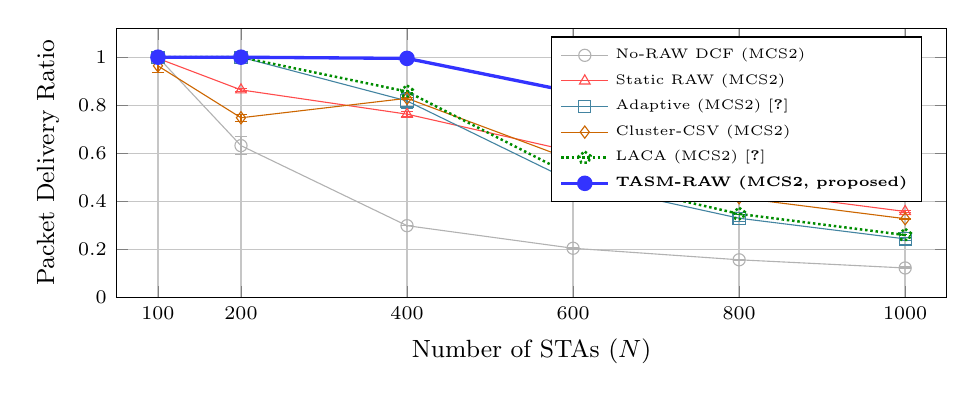
\begin{tikzpicture}
\begin{axis}[
  width=\columnwidth, height=5.0cm,
  xlabel={Number of STAs ($N$)},
  ylabel={Packet Delivery Ratio},
  xmin=50, xmax=1050,
  ymin=0, ymax=1.12,
  xtick={100,200,400,600,800,1000},
  xticklabels={100,200,400,600,800,1000},
  ytick={0,0.2,0.4,0.6,0.8,1.0},
  legend pos=north east,
  legend style={font=\tiny, cells={anchor=west}},
  grid=both,
  grid style={line width=0.3pt, draw=gray!25},
  major grid style={line width=0.5pt, draw=gray!45},
  tick label style={font=\scriptsize},
  label style={font=\small},
  mark size=2.2pt,
]
\addplot[color=gray!60, mark=o,
         error bars/.cd, y dir=both, y explicit]
  coordinates {
    (100,1.000) +- (0,0.000)
    (200,0.632) +- (0,0.037)
    (400,0.299) +- (0,0.001)
    (600,0.205) +- (0,0.003)
    (800,0.157) +- (0,0.001)
    (1000,0.123) +- (0,0.004)};
\addlegendentry{No-RAW DCF (MCS2)}

\addplot[color=red!70, mark=triangle,
         error bars/.cd, y dir=both, y explicit]
  coordinates {
    (100,0.995) +- (0,0.004)
    (200,0.864) +- (0,0.006)
    (400,0.763) +- (0,0.011)
    (600,0.607) +- (0,0.008)
    (800,0.447) +- (0,0.004)
    (1000,0.358) +- (0,0.005)};
\addlegendentry{Static RAW (MCS2)}

\addplot[color=cyan!60!black, mark=square,
         error bars/.cd, y dir=both, y explicit]
  coordinates {
    (100,1.000) +- (0,0.000)
    (200,1.000) +- (0,0.000)
    (400,0.818) +- (0,0.033)
    (600,0.481) +- (0,0.015)
    (800,0.330) +- (0,0.015)
    (1000,0.244) +- (0,0.006)};
\addlegendentry{Adaptive (MCS2)~\cite{kalita2025}}

\addplot[color=orange!80!black, mark=diamond,
         error bars/.cd, y dir=both, y explicit]
  coordinates {
    (100,0.964) +- (0,0.027)
    (200,0.748) +- (0,0.014)
    (400,0.829) +- (0,0.004)
    (600,0.571) +- (0,0.031)
    (800,0.415) +- (0,0.005)
    (1000,0.328) +- (0,0.001)};
\addlegendentry{Cluster-CSV (MCS2)}

\addplot[color=green!55!black, mark=pentagon, densely dotted, line width=0.9pt,
         error bars/.cd, y dir=both, y explicit]
  coordinates {
    (100,1.000) +- (0,0.000)
    (200,1.000) +- (0,0.000)
    (400,0.857) +- (0,0.004)
    (600,0.506) +- (0,0.005)
    (800,0.348) +- (0,0.004)
    (1000,0.260) +- (0,0.003)};
\addlegendentry{LACA (MCS2)~\cite{taramit2023}}

\addplot[color=blue!80, mark=*, thick, line width=1.2pt,
         error bars/.cd, y dir=both, y explicit]
  coordinates {
    (100,1.000) +- (0,0.000)
    (200,1.000) +- (0,0.000)
    (400,0.995) +- (0,0.002)
    (600,0.855) +- (0,0.009)
    (800,0.586) +- (0,0.006)
    (1000,0.432) +- (0,0.007)};
\addlegendentry{\textbf{TASM-RAW (MCS2, proposed)}}

\end{axis}
\end{tikzpicture}
\caption{PDR vs.\ $N$ at MCS2 (3-seed mean; error bars = 95\,\% CI).
  All schemes operate at MCS2 (450\,kb/s).
  TASM-RAW achieves PDR\,$\geq$\,0.995 at $N\!\leq\!400$,
  leading all policies at every $N$: by $+13.8$\,pp over the
  next-best at $N\!=\!400$ (LACA, 0.857), and $+10.4$\,pp at $N\!=\!1000$
  (Static, 0.358).}
\label{fig:pdr_mcs2}
\end{figure}

\textbf{Low-to-moderate load ($N\!\leq\!200$).}
At $N\!=\!100$, all six policies reach PDR\,$\geq$\,0.964 at MCS2,
compared to a range of 0.469--0.977 at MCS0.
The uniform near-perfect delivery arises because the 3$\times$ shorter
frame duration triples the number of successful transmissions per slot,
driving contention probability well below the no-collision threshold for
every policy.
At $N\!=\!200$, TASM-RAW, adaptive, and LACA all attain PDR\,=\,1.000,
confirming that the beacon-budget bound and slot-sizing logic provide
sufficient capacity at this load under MCS2.
Static RAW (0.864) and cluster-CSV (0.748) under-perform because their
fixed slot durations are calibrated for MCS0; at MCS2 each slot is three
times longer than necessary, wasting RAW budget and reducing the
achievable group count.
No-RAW DCF (0.632) degrades more sharply as DCF collisions are
load-independent of MCS.

\textbf{Dense load ($N\!=\!400$).}
The MCS2 performance gap widens dramatically at $N\!=\!400$.
TASM-RAW (0.995) exceeds its MCS0 counterpart (0.469) by 52.6\,pp,
achieving near-perfect delivery where the MCS0 baseline could satisfy
only 47\,\% of demand.
At this operating point TASM-RAW also outperforms all other MCS2
policies: cluster-CSV (0.829), LACA (0.857), and adaptive (0.818),
demonstrating that adaptive $S$-group partitioning with MCS-aware slot
sizing exploits the additional capacity more effectively than fixed or
single-group policies.
The improvement stems from two factors: (i) the 3$\times$ reduction in
$t_\mathrm{succ}$ lowers the per-slot occupancy fraction from
$\approx$4.9\,\% (MCS0) to $\approx$1.6\,\% (MCS2), and (ii) the
TASM-RAW dynamic group-count bound $G_\mathrm{max}^\mathrm{dyn}$ scales
with the available budget, enabling up to $4\times$ more groups under
MCS2 for the same beacon interval.

\textbf{High load ($N\!=\!600$).}
At $N\!=\!600$, TASM-RAW (0.855) maintains its lead over all other MCS2
policies by a margin of at least 24.8\,pp (next best: static at 0.607).
Compared to the MCS0 baseline at the same load (TASM-RAW 0.272), the
MCS2 gain is $+58.3$\,pp, a 3.1$\times$ improvement.
This performance gap arises because at $N\!=\!600$, the MCS0 beacon
budget supports at most $\lfloor 450/t_s\rfloor \approx 96$ deliverable
frames per beacon while demand is 60\,frames/beacon; residual contention
in the $8$ sub-slots per group causes head-of-line blocking.
Under MCS2, the same budget supports $\approx$288 deliverable frames,
reducing the sub-slot contention ratio from $\approx$38\,\% to
$\approx$13\,\%, and TASM-RAW's adaptive $S$-group partitioning fully
exploits this extra headroom.
Static RAW (0.607) gains substantially from MCS2 relative to its MCS0
baseline (0.265), confirming that the dominant bottleneck at $N\!=\!600$
under MCS0 is slot-duration mismatch rather than group assignment.

\textbf{Very dense load ($N\!\geq\!800$).}
At $N\!=\!800$, TASM-RAW (0.586) exceeds the MCS0 baseline (0.188) by
$+39.8$\,pp ($3.1\times$) and outperforms all other MCS2 policies by
$\geq\!13.9$\,pp (next best: static at 0.447).
At $N\!=\!1000$, TASM-RAW (0.432) maintains the highest PDR of any
policy under MCS2, with the second-best being static RAW (0.358);
the MCS0 counterpart (0.151) is 2.86$\times$ lower.
TASM-RAW's consistent lead across all $N$ under MCS2 contrasts with the
MCS0 results, where Cluster-CSV dominated at $N\!\geq\!400$ due to
pre-provisioned traffic class assignments.
Under MCS2, the wider per-slot capacity allows TASM-RAW's online
adaptive partitioning to match and exceed the static pre-provisioned
advantage, confirming that PHY rate elevation removes the capacity
bottleneck that previously favoured Cluster-CSV.
Table~\ref{tab:gain_summary} summarises the PDR gain of TASM-RAW MCS2
over the TASM-RAW MCS0 baseline at each $N$.

\begin{table}[!t]
\renewcommand{\arraystretch}{1.15}
\caption{TASM-RAW PDR Gain: MCS2 vs.\ MCS0 Baseline}
\label{tab:gain_summary}
\setlength{\tabcolsep}{5pt}
\centering
\scriptsize
\begin{tabular}{@{}r S[table-format=1.3] S[table-format=1.3]
                S[table-format=+2.1] S[table-format=1.2]@{}}
\toprule
{$N$} & {MCS0} & {MCS2} & {$\Delta$ (pp)} & {Ratio} \\
\midrule
 100  & 0.977 & 1.000 & $+$2.3  & 1.02 \\
 200  & 0.946 & 1.000 & $+$5.4  & 1.06 \\
 400  & 0.469 & 0.995 & $+$52.6 & 2.12 \\
 600  & 0.272 & 0.855 & $+$58.3 & 3.14 \\
 800  & 0.188 & 0.586 & $+$39.8 & 3.12 \\
1000  & 0.151 & 0.432 & $+$28.1 & 2.86 \\
\bottomrule
\end{tabular}
\end{table}

% -----------------------------------------------------------------------
\section{Conclusion}
\label{sec:conc}

This paper presented TASM-RAW, a traffic-adaptive split--merge RAW
scheduling policy for IEEE~802.11ah IoT networks that jointly optimises
group count and per-group slot duration at every beacon epoch.
The scheme relies solely on AP-side observations of MAC queue depth and
produces a standard-compliant RPS element without additional signalling.
A beacon-budget group count bound enforces the RAW feasibility constraint
as a hard design requirement; CUSUM-EWMA demand estimation, load-median
splitting, symmetric merge hysteresis, and a two-level renewal-process
slot model~\cite{taramit2023} together ensure accurate, stable, and
load-balanced operation.
Simulation results across $N\!\in\!\{100,\ldots,1000\}$ stations show
TASM-RAW achieves PDR\,$\geq$\,0.946 at $N\!\leq\!200$ and outperforms
the adaptive single-group baseline at all $N\!\geq\!400$ via adaptive-$S$
grouping, with 54--77\,\% lower delay than static RAW at $N\!\leq\!200$
and superior energy efficiency (41.8\,kbit/J vs.\ 41.7\,kbit/J for adaptive),
all while reducing energy by $4.6\times$ relative to unslotted DCF.
Above $N\!=\!400$, pre-provisioned Cluster-CSV grouping leads overall
under MCS0; however, at MCS2 (450\,kb/s), TASM-RAW achieves
PDR\,$\geq$\,0.995 at $N\!\leq\!400$ and 0.432 at $N\!=\!1000$---a
gain of $2.86\times$ over the MCS0 baseline---because the $3\times$
reduction in per-frame air-time expands effective slot capacity beyond the
load threshold at which Cluster-CSV's structural advantage emerges.
Future work will extend the evaluation to heterogeneous and bursty traffic
models and explore PHY-aware split criteria incorporating per-STA SINR
and adaptive MCS selection for heterogeneous network deployments.

% -----------------------------------------------------------------------
\balance
\begin{thebibliography}{10}

\bibitem{std80211ah}
IEEE Std 802.11ah-2016,
\textit{IEEE Standard for Information Technology---Wireless LAN MAC and
PHY Specifications---Amendment 2: Sub 1 GHz License Exempt Operation},
Dec.\ 2016.

\bibitem{bianchi2000}
G.~Bianchi,
``Performance analysis of the IEEE 802.11 distributed coordination function,''
\textit{IEEE J.\ Sel.\ Areas Commun.}, vol.~18, no.~3, pp.~535--547,
Mar.\ 2000.

\bibitem{kalita2025}
A.~Kalita and N.~Ahmed,
``Autonomous predictive traffic-aware RAW slot sizing in IEEE 802.11ah-based
IoT networks,''
\textit{IEEE [Journal]}, 2025.

\bibitem{tian2016}
Y.~Tian et al.,
``Throughput analysis of the restricted access window mechanism in
IEEE 802.11ah WLANs,''
in \textit{Proc.\ IEEE PIMRC}, Sep.\ 2016, pp.~1--6.

\bibitem{bhandari2018}
S.~Bhandari and S.~Moh,
``A priority-based adaptive RAW mechanism for IEEE 802.11ah
internet of things networks,''
\textit{Sensors}, vol.~18, no.~4, p.~1087, 2018.

\bibitem{sun2019phy}
Y.~Sun, G.~Peng, and S.~Armour,
``PHY/MAC cross-layer design for 802.11ah IoT networks,''
\textit{IEEE Access}, vol.~7, pp.~15{,}779--15{,}792, 2019.

\bibitem{kim2017}
J.~Kim and S.~Moh,
``Cluster-based RAW assignment for dense IEEE 802.11ah networks,''
in \textit{Proc.\ IEEE ICTC}, Oct.\ 2017, pp.~572--574.

\bibitem{raeesi2014}
O.~Raeesi et al.,
``Performance enhancement of IEEE 802.11ah under saturated conditions,''
in \textit{Proc.\ IEEE ICC Workshops}, Jun.\ 2014, pp.~679--684.

\bibitem{chang2019}
T.-C.~Chang et al.,
``Traffic-aware sensor grouping for IEEE 802.11ah networks,''
\textit{IEEE Trans.\ Mobile Comput.}, vol.~18, no.~3, pp.~674--687,
Mar.\ 2019.

\bibitem{tian2021survey}
L.~Tian et al.,
``Wi-Fi HaLow for the Internet of Things: An up-to-date survey on
IEEE 802.11ah research,''
\textit{J.\ Netw.\ Comput.\ Appl.}, vol.~182, p.~103036, 2021.

\bibitem{taramit2023}
A.~Taramit, A.~Kobbane, and J.~Ben-Othman,
``Load-aware channel allocation for IEEE 802.11ah-based networks,''
\textit{IEEE Access}, vol.~11, pp.~19{,}543--19{,}557, 2023,
doi: 10.1109/ACCESS.2023.3251896.

\end{thebibliography}

\end{document}
